\documentclass[12pt,letterpaper]{article}
\usepackage{graphicx,textcomp}
\usepackage{natbib}
\usepackage{setspace}
\usepackage{fullpage}
\usepackage{color}
\usepackage[reqno]{amsmath}
\usepackage{amsthm}
\usepackage{fancyvrb}
\usepackage{amssymb,enumerate}
\usepackage[all]{xy}
\usepackage{endnotes}
\usepackage{lscape}
\newtheorem{com}{Comment}
\usepackage{float}
\usepackage{hyperref}
\newtheorem{lem} {Lemma}
\newtheorem{prop}{Proposition}
\newtheorem{thm}{Theorem}
\newtheorem{defn}{Definition}
\newtheorem{cor}{Corollary}
\newtheorem{obs}{Observation}
\usepackage[compact]{titlesec}
\usepackage{dcolumn}
\usepackage{tikz}
\usetikzlibrary{arrows}
\usepackage{multirow}
\usepackage{xcolor}
\newcolumntype{.}{D{.}{.}{-1}}
\newcolumntype{d}[1]{D{.}{.}{#1}}
\definecolor{light-gray}{gray}{0.65}
\usepackage{url}
\usepackage{listings}
\usepackage{color}

\definecolor{codegreen}{rgb}{0,0.6,0}
\definecolor{codegray}{rgb}{0.5,0.5,0.5}
\definecolor{codepurple}{rgb}{0.58,0,0.82}
\definecolor{backcolour}{rgb}{0.95,0.95,0.92}

\lstdefinestyle{mystyle}{
	backgroundcolor=\color{backcolour},   
	commentstyle=\color{codegreen},
	keywordstyle=\color{magenta},
	numberstyle=\tiny\color{codegray},
	stringstyle=\color{codepurple},
	basicstyle=\footnotesize,
	breakatwhitespace=false,         
	breaklines=true,                 
	captionpos=b,                    
	keepspaces=true,                 
	numbers=left,                    
	numbersep=5pt,                  
	showspaces=false,                
	showstringspaces=false,
	showtabs=false,                  
	tabsize=2
}
\lstset{style=mystyle}
\newcommand{\Sref}[1]{Section~\ref{#1}}
\newtheorem{hyp}{Hypothesis}

\title{Problem Set 3}
\date{Due: November 11, 2024}
\author{Applied Stats/Quant Methods 1}


\begin{document}
	\maketitle
	\section*{Instructions}
	\begin{itemize}
		\item Please show your work! You may lose points by simply writing in the answer. If the problem requires you to execute commands in \texttt{R}, please include the code you used to get your answers. Please also include the \texttt{.R} file that contains your code. If you are not sure if work needs to be shown for a particular problem, please ask.
	\item Your homework should be submitted electronically on GitHub.
	\item This problem set is due before 23:59 on Sunday November 11, 2024. No late assignments will be accepted.

	\end{itemize}

		\vspace{.25cm}
	
\noindent In this problem set, you will run several regressions and create an add variable plot (see the lecture slides) in \texttt{R} using the \texttt{incumbents\_subset.csv} dataset. Include all of your code.

	\vspace{.5cm}
\section*{Question 1}
\vspace{.25cm}
\noindent We are interested in knowing how the difference in campaign spending between incumbent and challenger affects the incumbent's vote share. 
	\begin{enumerate}
		\item Run a regression where the outcome variable is \texttt{voteshare} and the explanatory variable is \texttt{difflog}.	\vspace{5cm}
		\lstinputlisting[language=R, firstline=34, lastline=37]{"C:\\Users\\User\\Desktop\\my_answers\\PS3_answers.R"}
		\vspace{0.2cm}
		\begin{verbatim}
			Call:
			lm(formula = voteshare ~ difflog, data = inc.sub)
			
			Residuals:
			Min       1Q   Median       3Q      Max 
			-0.26832 -0.05345 -0.00377  0.04780  0.32749 
			
			Coefficients:
			Estimate Std. Error t value Pr(>|t|)    
			(Intercept) 0.579031   0.002251  257.19   <2e-16 ***
			difflog     0.041666   0.000968   43.04   <2e-16 ***
			---
			Signif. codes:  0 ‘***’ 0.001 ‘**’ 0.01 ‘*’ 0.05 ‘.’ 0.1 ‘ ’ 1
			
			Residual standard error: 0.07867 on 3191 degrees of freedom
			Multiple R-squared:  0.3673,	Adjusted R-squared:  0.3671 
			F-statistic:  1853 on 1 and 3191 DF,  p-value: < 2.2e-16
		\end{verbatim}
		overall the model explains the difference in campaign spend between incumbents and challengers have a statistically significant and positive effect on vote share, with 36.73 percent of the variance in vote share explained by campaign spending differences.
		\vspace{.25cm}
		\item Make a scatterplot of the two variables and add the regression line. 	\vspace{0.7cm}
		\lstinputlisting[language=R, firstline=41, lastline=44]{"C:\\Users\\User\\Desktop\\my_answers\\PS3_answers.R"}
		\vspace{7.1cm}
			\begin{figure}[h!]
			\centering
			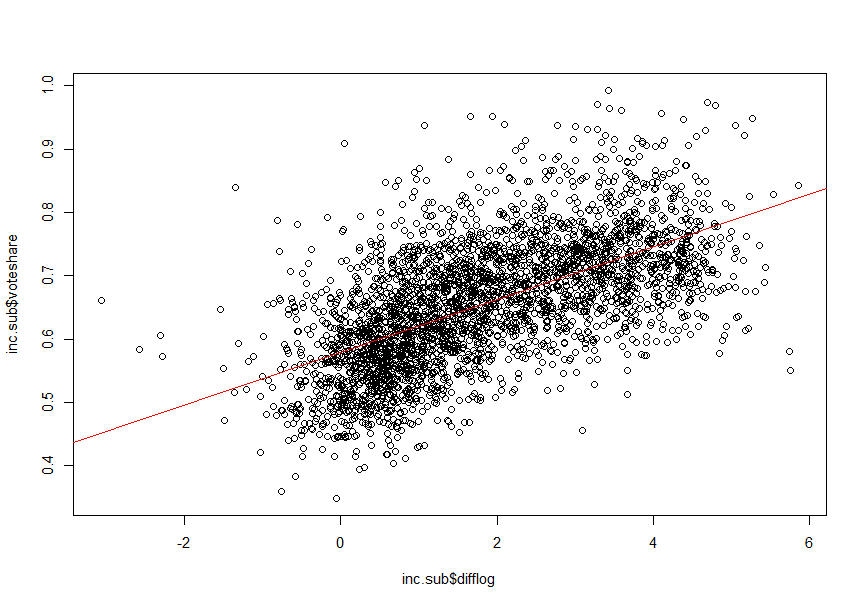
\includegraphics[width=.85\textwidth]{"C:\\Users\\User\\Desktop\\my_answers\\plot_3_1.png"}
			\caption{Scatterplot of difflog vs. voteshare with regression line}
			\label{fig:plot_1}
		\end{figure}
		
		\vspace{.25cm}
	\end{enumerate}
	 \begin{enumerate}
	 	3. Save the residuals of the model in a separate object.	\vspace{0.2cm}
	 	\lstinputlisting[language=R, firstline=48, lastline=49]{"C:\\Users\\User\\Desktop\\my_answers\\PS3_answers.R"}
	
	 	4. Write the prediction equation
	 	\vspace{.25cm}
	 	\begin{equation}
	 		\ y = \beta_0 + \beta_1 x
	 	\end{equation}
	 	\begin{itemize}
	 	\item \( y \): voteshare
	 	\item \(\beta_0\): intercept
	 	\item \(\beta_1 \): slope
	 	\item \( x \): difflog
	 	\end{itemize}
	 	\begin{equation}
	 		voteshare = 0.579031+0.041666*difflog
	 	\end{equation}
	 	\lstinputlisting[language=R, firstline=53, lastline=57]{"C:\\Users\\User\\Desktop\\my_answers\\PS3_answers.R"}
	 	\end{enumerate}
	
\newpage

\section*{Question 2}
\noindent We are interested in knowing how the difference between incumbent and challenger's spending and the vote share of the presidential candidate of the incumbent's party are related.	\vspace{.25cm}
\begin{enumerate}
	\item Run a regression where the outcome variable is `presvote` and the explanatory variable is `difflog`.
	
	\vspace{0.5cm}
	
	\lstinputlisting[language=R, firstline=62, lastline=65]{"C:\\Users\\User\\Desktop\\my_answers\\PS3_answers.R"}
	
	\begin{verbatim}
	Call:
	lm(formula = presvote ~ difflog, data = inc.sub)
	
	Residuals:
	Min       1Q   Median       3Q      Max 
	-0.32196 -0.07407 -0.00102  0.07151  0.42743 
	
	Coefficients:
	Estimate Std. Error t value Pr(>|t|)    
	(Intercept) 0.507583   0.003161  160.60   <2e-16 ***
	difflog     0.023837   0.001359   17.54   <2e-16 ***
	---
	Signif. codes:  0 ‘***’ 0.001 ‘**’ 0.01 ‘*’ 0.05 ‘.’ 0.1 ‘ ’ 1
	
	Residual standard error: 0.1104 on 3191 degrees of freedom
	Multiple R-squared:  0.08795,	Adjusted R-squared:  0.08767 
	F-statistic: 307.7 on 1 and 3191 DF,  p-value: < 2.2e-16
	\end{verbatim}
	Overall, the model shows that the difference in campaign spending between incumbents and challengers has a statistically significant and positive effect on the presidential candidate's vote share. However, only 8.7 percent of the variance in the presidential vote share is explained by campaign spending differences. Specifically, a one-unit increase in the difference in campaign spending between the incumbent and challenger leads to a 2.38 percentage point increase in the presidential vote share. The low R-squared value indicates that campaign spending is not a strong predictor of presidential vote share.
	
	\item Make a scatterplot of the two variables and add the regression line.
	\vspace{0.5cm}
	
	\lstinputlisting[language=R, firstline=68, lastline=70]{"C:\\Users\\User\\Desktop\\my_answers\\PS3_answers.R"}
	
	\begin{figure}[h!]
		\centering
		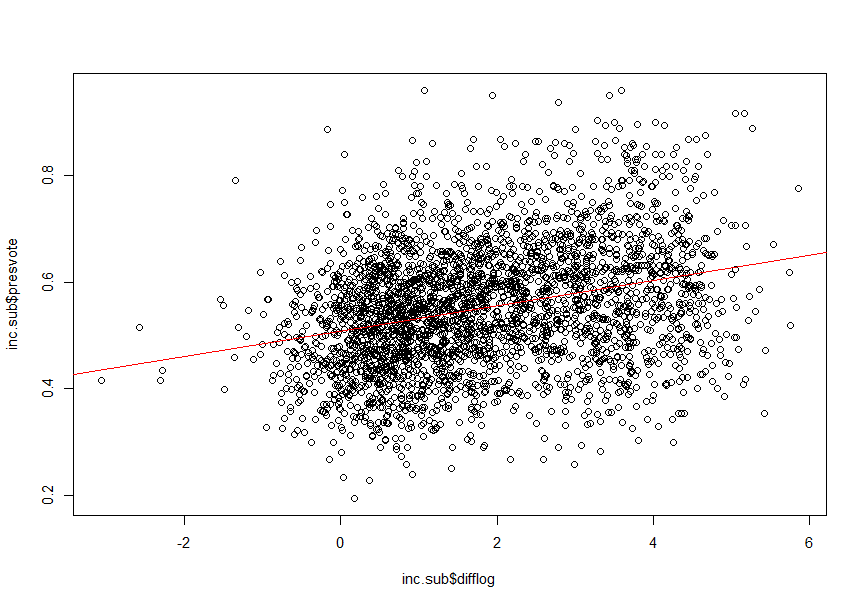
\includegraphics[width=.85\textwidth]{"C:\\Users\\User\\Desktop\\my_answers\\plot_3_2.png"}
		\caption{Scatterplot of presvote vs. difflog with regression line}
		\label{fig:plot_2}
	\end{figure}
	
	\vspace{10cm}
	\item Save the residuals of the model in a separate object.
	\vspace{0.5cm}
	\lstinputlisting[language=R, firstline=73, lastline=75]{"C:\\Users\\User\\Desktop\\my_answers\\PS3_answers.R"}
	
	\item Write the prediction equation.
	\begin{equation}
		y = \beta_0 + \beta_1 x
	\end{equation}
	\begin{itemize}
		\item \( y \): presvote
		\item \(\beta_0\): intercept
		\item \(\beta_1 \): slope
		\item \( x \): difflog
	\end{itemize}
	\begin{equation}
		presvote = 0.507583+0.023837*difflog
	\end{equation}
	\lstinputlisting[language=R, firstline=77, lastline=81]{"C:\\Users\\User\\Desktop\\my_answers\\PS3_answers.R"}
	
\end{enumerate}
	
	\newpage	
\section*{Question 3}

\noindent We are interested in knowing how the vote share of the presidential candidate of the incumbent's party is associated with the incumbent's electoral success.
	\vspace{.25cm}
	\begin{enumerate}
		\item Run a regression where the outcome variable is
		 \texttt{voteshare} and the explanatory variable is \texttt{presvote}.
		 \lstinputlisting[language=R, firstline=86, lastline=87]{"C:\\Users\\User\\Desktop\\my_answers\\PS3_answers.R"}
	\begin{Verbatim}
 	> summary(model_3)
 	
 	Call:
 	lm(formula = voteshare ~ presvote, data = inc.sub)
 	
 	Residuals:
 	Min       1Q   Median       3Q      Max 
 	-0.27330 -0.05888  0.00394  0.06148  0.41365 
 	
 	Coefficients:
 	            Estimate Std. Error t value Pr(>|t|)    
 	(Intercept) 0.441330   0.007599   58.08   <2e-16 ***
 	presvote    0.388018   0.013493   28.76   <2e-16 ***
 	---
 	Signif. codes:  0 ‘***’ 0.001 ‘**’ 0.01 ‘*’ 0.05 ‘.’ 0.1 ‘ ’ 1
 	
 	Residual standard error: 0.08815 on 3191 degrees of freedom
 	Multiple R-squared:  0.2058,	Adjusted R-squared:  0.2056 
 	F-statistic:   827 on 1 and 3191 DF,  p-value: < 2.2e-16
 	
	\end{Verbatim}
	Overall, the model shows that presvote (presidential vote share) has a statistically significant effect on voteshare (the vote share of the incumbent's party). 20.58 percent  of the variance in the vote share is explained by presvote. Specifically, a one-unit increase in presvote leads to a 38.8 percentage point increase in the voteshare.
			\vspace{0.5cm}
		\item Make a scatterplot of the two variables and add the regression line.
		\lstinputlisting[language=R, firstline=90, lastline=93]{"C:\\Users\\User\\Desktop\\my_answers\\PS3_answers.R"}
			\vspace{0.5cm}
			\begin{figure}[h!]
				\centering
			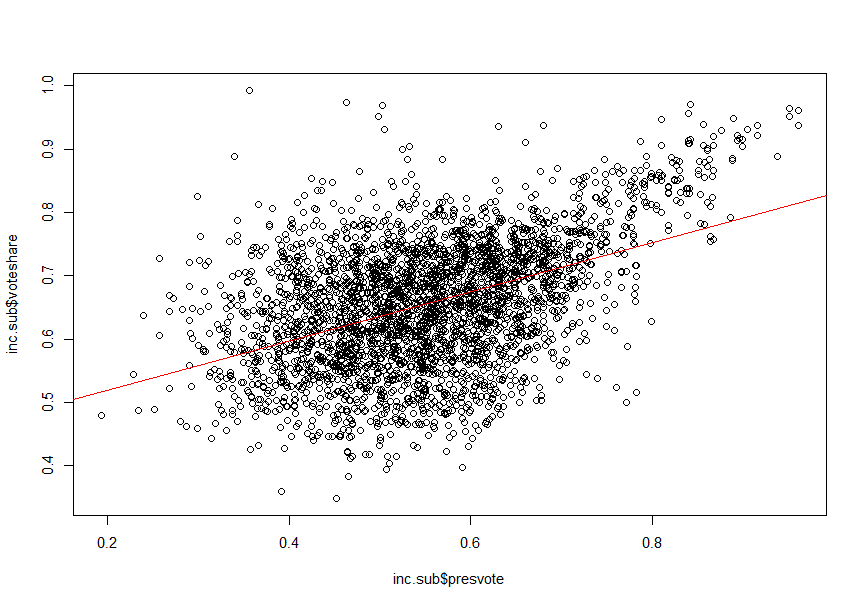
\includegraphics[width=.85\textwidth]{"C:\\Users\\User\\Desktop\\my_answers\\plot_3_3.png"}
			\caption{Scatterplot of voteshare vs. presvote with regression line}
			\label{fig:plot_3}
			\end{figure}
			\vspace{10cm}
		\item Write the prediction equation.
		\vspace{.25cm}
		\begin{equation}
			\ y = \beta_0 + \beta_1 x
			\end{equation}
			\begin{itemize}
				\item \( y \): voteshare
				\item \(\beta_0\): intercept
				\item \(\beta_1 \): slope
				\item \( x \): presvote
			\end{itemize}
			\begin{equation}
				voteshare = 0.441330+0.388018*presvote
			\end{equation}
		\lstinputlisting[language=R, firstline=96, lastline=100]{"C:\\Users\\User\\Desktop\\my_answers\\PS3_answers.R"}
	\end{enumerate}
	

\newpage	
\section*{Question 4}
\noindent The residuals from part (a) tell us how much of the variation in \texttt{voteshare} is $not$ explained by the difference in spending between incumbent and challenger. The residuals in part (b) tell us how much of the variation in \texttt{presvote} is $not$ explained by the difference in spending between incumbent and challenger in the district.
	\begin{enumerate}
		\item Run a regression where the outcome variable is the residuals from Question 1 and the explanatory variable is the residuals from Question 2.	\vspace{0.2cm}
		\lstinputlisting[language=R, firstline=104, lastline=105]{"C:\\Users\\User\\Desktop\\my_answers\\PS3_answers.R"}
		\begin{Verbatim}
Call:
lm(formula = model_residuals ~ model_residual_2, data = inc.sub)

Residuals:
Min       1Q   Median       3Q      Max 
-0.25928 -0.04737 -0.00121  0.04618  0.33126 

Coefficients:
Estimate Std. Error t value Pr(>|t|)    
(Intercept)      -5.934e-18  1.299e-03    0.00        1    
model_residual_2  2.569e-01  1.176e-02   21.84   <2e-16 ***
---
Signif. codes:  0 ‘***’ 0.001 ‘**’ 0.01 ‘*’ 0.05 ‘.’ 0.1 ‘ ’ 1

Residual standard error: 0.07338 on 3191 degrees of freedom
Multiple R-squared:   0.13,	Adjusted R-squared:  0.1298 
F-statistic:   477 on 1 and 3191 DF,  p-value: < 2.2e-16

		\end{Verbatim}
		The model indicates a statistically significant effect of the residuals of presvote on the residuals of voteshare, with 13 percent of the variance in the voteshare residuals explained by the presvote residuals. The positive coefficient of 0.256 suggests that as the residuals of presvote increase, the residuals of voteshare also tend to increase.
		\item Make a scatterplot of the two residuals and add the regression line. 
		\lstinputlisting[language=R, firstline=108, lastline=109]{"C:\\Users\\User\\Desktop\\my_answers\\PS3_answers.R"}
		\begin{figure}[h!]
			\centering
			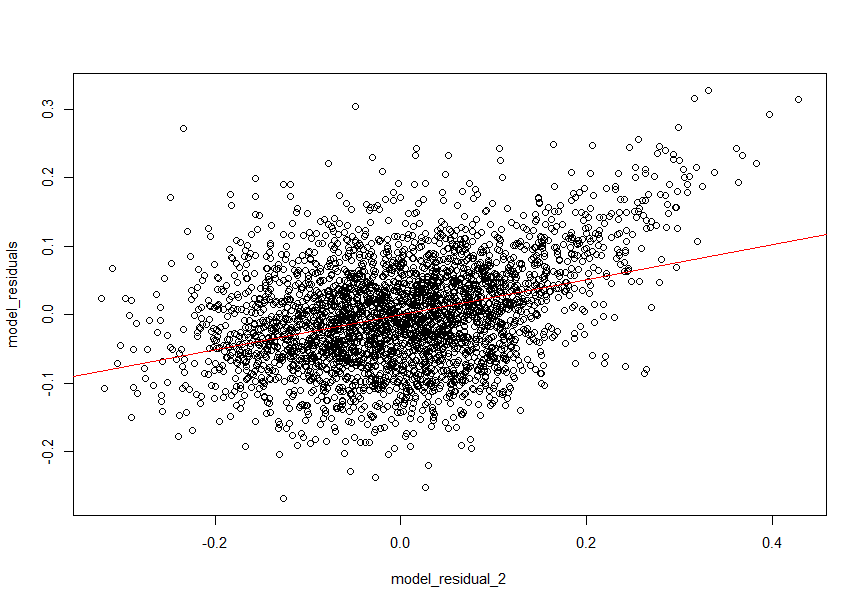
\includegraphics[width=.85\textwidth]{"C:\\Users\\User\\Desktop\\my_answers\\plot_3_4.png"}
			\caption{Scatterplot of model residual 2 vs. model residual with regression line}
			\label{fig:plot_2}
		\end{figure}
			\vspace{6cm}
		\item Write the prediction equation.
			\begin{equation}
			\ y = \beta_0 + \beta_1 x
		\end{equation}
		\begin{itemize}
			\item \( y \): residuals of voteshare
			\item \(\beta_0\): intercept
			\item \(\beta_1 \): slope
			\item \( x \): residuals of presvote
			\end{itemize}
			\begin{equation}
				\text{model\_residuals} = -5.934e-18+2.569e-01*\text{model\_residual\_2}
			\end{equation}
		\lstinputlisting[language=R, firstline=112, lastline=116]{"C:\\Users\\User\\Desktop\\my_answers\\PS3_answers.R"}
		
		
		
	\end{enumerate}
	
	\newpage	

\section*{Question 5}
\noindent What if the incumbent's vote share is affected by both the president's popularity and the difference in spending between incumbent and challenger? 
	\begin{enumerate}
		\item Run a regression where the outcome variable is the incumbent's \texttt{voteshare} and the explanatory variables are \texttt{difflog} and \texttt{presvote}.
		\lstinputlisting[language=R, firstline=121, lastline=122]{"C:\\Users\\User\\Desktop\\my_answers\\PS3_answers.R"}
		\begin{verbatim}
		lm(formula = voteshare ~ difflog + presvote, data = inc.sub)
		
		Residuals:
		Min       1Q   Median       3Q      Max 
		-0.25928 -0.04737 -0.00121  0.04618  0.33126 
		
		Coefficients:
	            	Estimate Std. Error t value Pr(>|t|)    
		(Intercept) 0.4486442  0.0063297   70.88   <2e-16 ***
		difflog     0.0355431  0.0009455   37.59   <2e-16 ***
		presvote    0.2568770  0.0117637   21.84   <2e-16 ***
		---
		Signif. codes:  0 ‘***’ 0.001 ‘**’ 0.01 ‘*’ 0.05 ‘.’ 0.1 ‘ ’ 1
		
		Residual standard error: 0.07339 on 3190 degrees of freedom
		Multiple R-squared:  0.4496,	Adjusted R-squared:  0.4493 
		F-statistic:  1303 on 2 and 3190 DF,  p-value: < 2.2e-16
		\end{verbatim}
		here the multiple regression model  suggests that both difflog (the difference in campaign spending) and presvote (the presidential vote share) are statistically significant predictors of incumbent's voteshare, where a one unit increase in difflog leads to 3.55 percent increase in voteshare, and a one unit increase in presvote leads to 25.68 percentage increase in voteshare. overall 44.93 percentage of variance in voteshare can be explained by both the predictors.
		\vspace{0.2cm}
		\item Write the prediction equation.
		\begin{equation}
			\ y = \beta_0 + \beta_1 x_1+\beta_2 x_2
		\end{equation}
		\begin{itemize}
				\item \( y \): voteshare
				\item \(\beta_0\): intercept
				\item \(\beta_1 \): coefficient. of difflog
				\item \(\beta_1 \): coefficient of presvote
				\item \( x_1 \): difflog
				\item \( x_2 \): presvote
				\end{itemize}
			\begin{equation}
				voteshare= 0.4486442+0.0355431*difflog+0.2568770*presvote
			\end{equation}
			\lstinputlisting[language=R, firstline=125, lastline=131]{"C:\\Users\\User\\Desktop\\my_answers\\PS3_answers.R"}
			\vspace{0.2cm}
		\item What is it in this output that is identical to the output in Question 4? Why do you think this is the case?
		\begin{itemize}
			\item \textbf{Common Residuals}
			\newline
			In Model 4, we used the residuals of presvote and voteshare to model their relationship. inorder to explain the  variations in voteshare using the residuals of presvote. In Model 5, presvote is used as an independent variable in a multiple regression model with voteshare as the dependent variable. Because both models work with voteshare's unexplained variance, they end up with similar residuals. Therefore a common residuals in bot the models are observed,as both involve capturing variations in voteshare associated with presvote.
			\vspace{0.2cm}
			\item\textbf{Coeffiecnts of prevote}
			\newline
			In Model 4, the residuals of presvote were used as the independent variable to explain the residuals of voteshare, while in Model 5, presvote itself is one of the predictors for voteshare. Since residuals of presvote in Model 4 help explain voteshare residuals, and presvote itself is a predictor in Model 5, thereby leading to a similar pattern in coefficients. there exists a strong effect of presvote on voteshare in both the models, with a significant p-value (< 2e-16).
			\vspace{0.2cm}
			\item \textbf{Standardsied residuals }
			\newline
			Both models analyze the residuals of voteshare, which is why they show similar standard residual errors. In each model, the residuals represent the remaining variance in voteshare after accounting for the independent variables. Both models are designed to capture how presvote impacts voteshare: directly in Model 5 as an independent variable, and indirectly in Model 4 through the residuals of presvote. therefore similar standardized residual errors across the two models.
			
			In conclusion, presvote has a statistically significant positive effect on vote share.
			
		\end{itemize}
			
		
		 
	\end{enumerate}




\end{document}
